\section{Guidelines}
The development of the UI must follow a series of general guidelines:
\begin{itemize}
 \item Keep the UI as simple as possible (avoid bloat)
 \item The UI must be as intuitive as possible
 \item The user experience must be as consistent as possible, even across different devices
\end{itemize}

\section{Mockup}
Additionally, the following mock-ups are provided, in aid to the ui implementation.
\begin{figure} [h]
\centering
  	  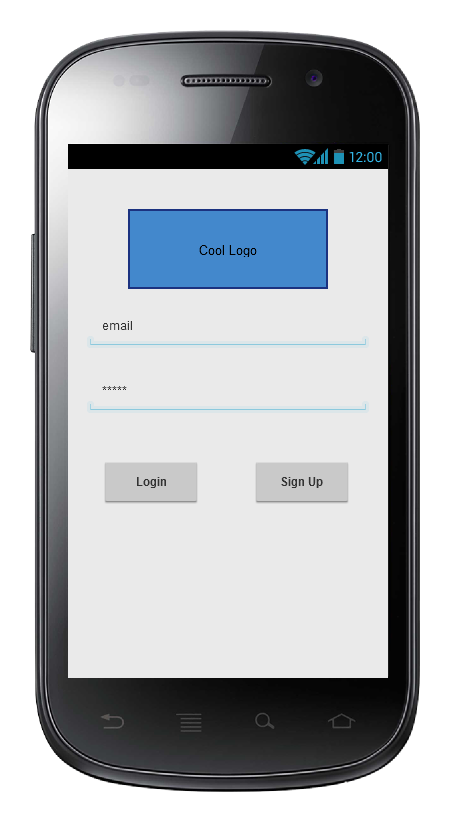
\includegraphics[scale=0.5]{../RASD/ui/sequencelogin.png}
\caption{Login}
\end{figure}

\begin{figure} [h]
\centering
  	  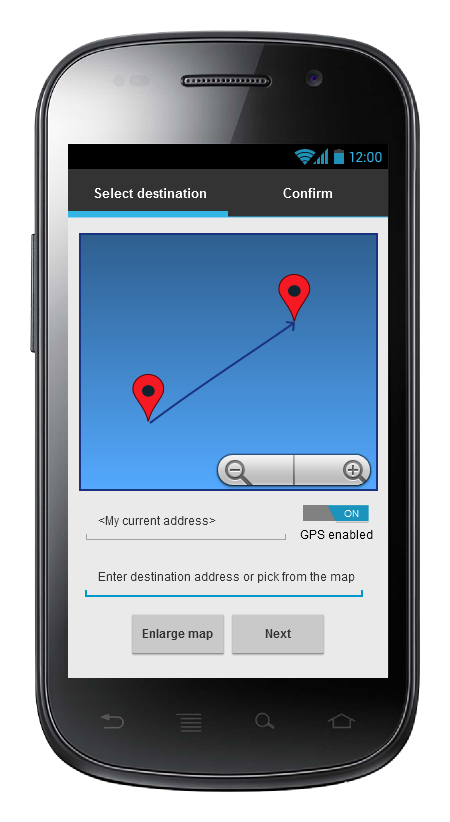
\includegraphics[scale=0.5]{../RASD/ui/Passenger map screen.png}
\caption{Passenger map screen}
\end{figure}

\begin{figure} [h]
\centering
  	  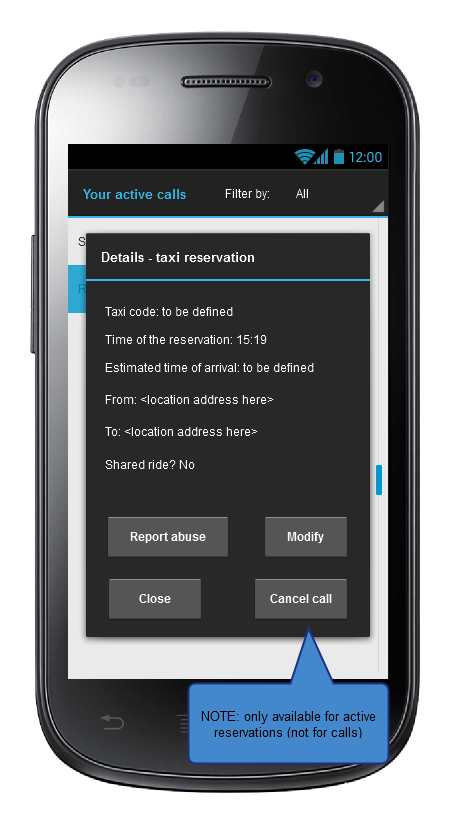
\includegraphics[scale=0.5]{../RASD/ui/Passenger call list detail.png}
\caption{Passenger call list detail}
  
	\end{figure}
	
\begin{figure} [h]
\centering
  	  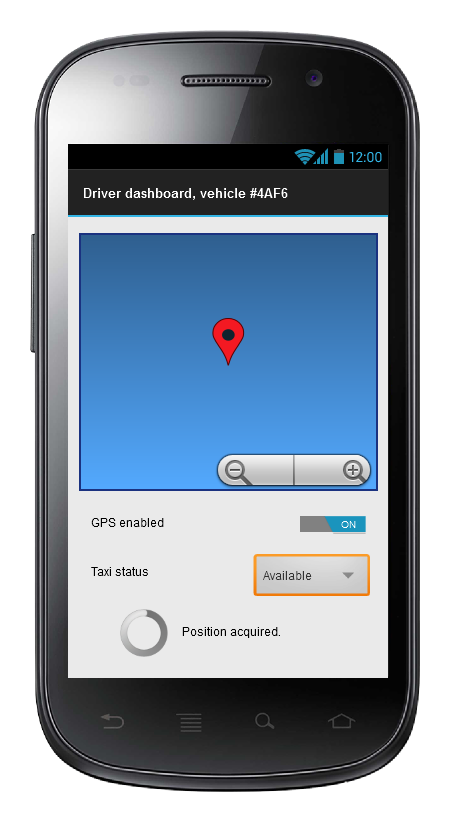
\includegraphics[scale=0.5]{../RASD/ui/Driver Idle screen.png}
\caption{Driver Idle screen}
    
	\end{figure}
\begin{figure} [h]
\centering
  	  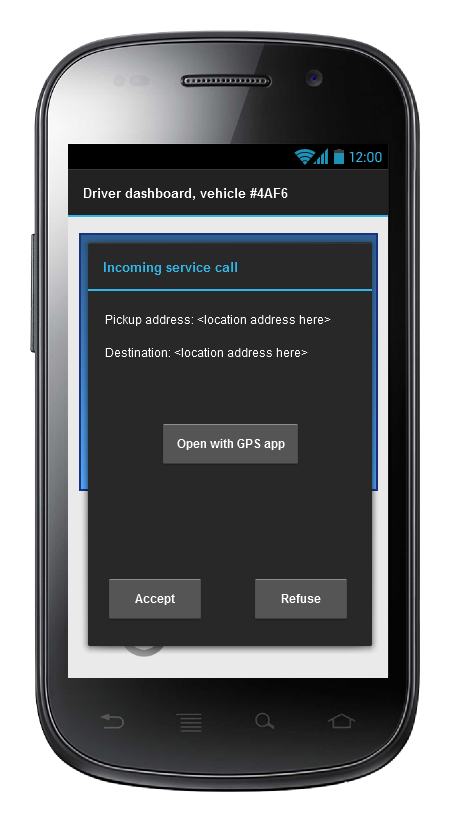
\includegraphics[scale=0.5]{../RASD/ui/Driver new call dialog.png}
\caption{Driver new call dialog}
    
	\end{figure}

\begin{figure} [h]
\centering
  	  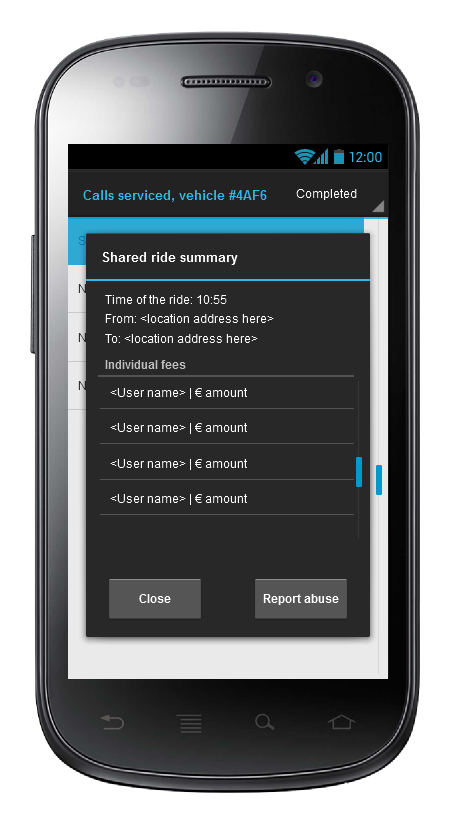
\includegraphics[scale=0.5]{../RASD/ui/Driver shared fee dialog.png}
\caption{Driver shared fee dialog}
    
	\end{figure}
